\documentclass{article}
\usepackage[pdftex]{graphicx}
\usepackage{amsmath}
\usepackage{verbatim}
\usepackage{enumerate}
\author{Michael Anderson}
\title{Homework 3}
\begin{document}
\maketitle
\center{CS517}
\center{Prof. Cull}\\
\flushleft
\newpage

\section{}
We could argue that since an $n$ has been found for all of the trillions of
natural numbers already tried, probably no natural number will be found that
does not map to 1 eventually upon successive applications of the Collatz
function. Therefore a program that returns an answer to the question: ``Do all
natural numbers eventually map to 1 upon successive applications of the
Collatz function" could be:

\begin{verbatim} RETURN YES \end{verbatim}

If during the generation of the Collatz sequence for some $x$, a cycle is
entered (which would preclude $x$ ever reaching 1),
then the program could return NO. So
another possible one-liner (easily implementable as an actual one-liner in a
language such as Haskell or J) would be:

\begin{verbatim}
Iterate through the naturals until a Collatz sequence is found for one of them
 that enters into a cycle, and then return NO.
\end{verbatim}

It turns out that in practice that the amount of time and space required to
actually get an answer from the above program is very problematic.

\section{}
collatz.py is attached.

\section{}
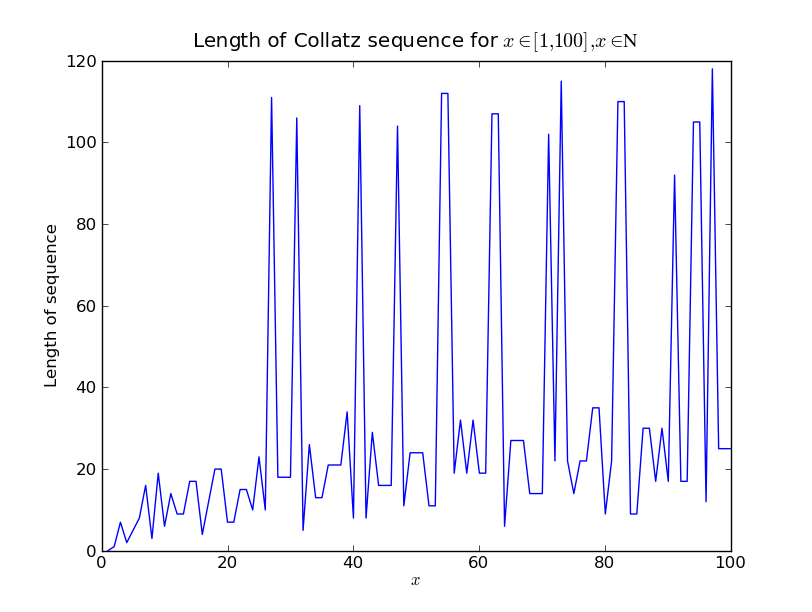
\includegraphics[scale=0.5]{col100.png}
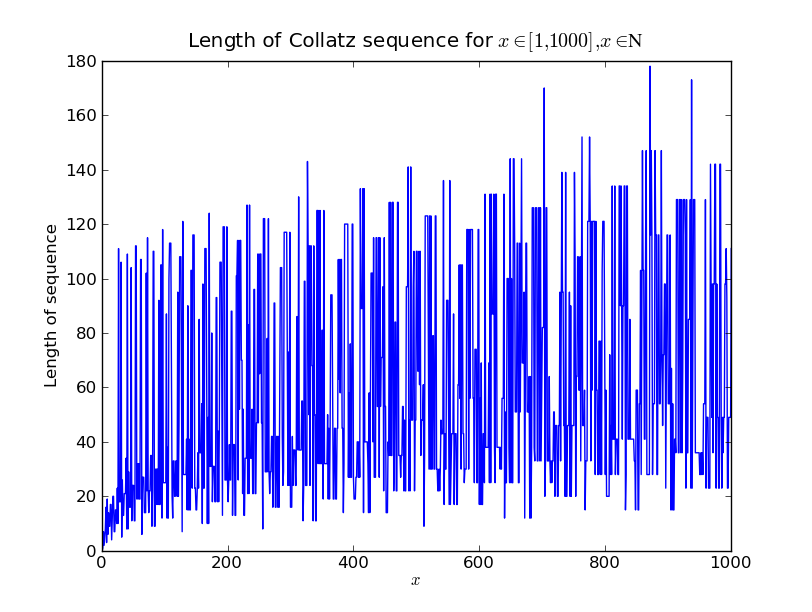
\includegraphics[scale=0.5]{col1000.png}
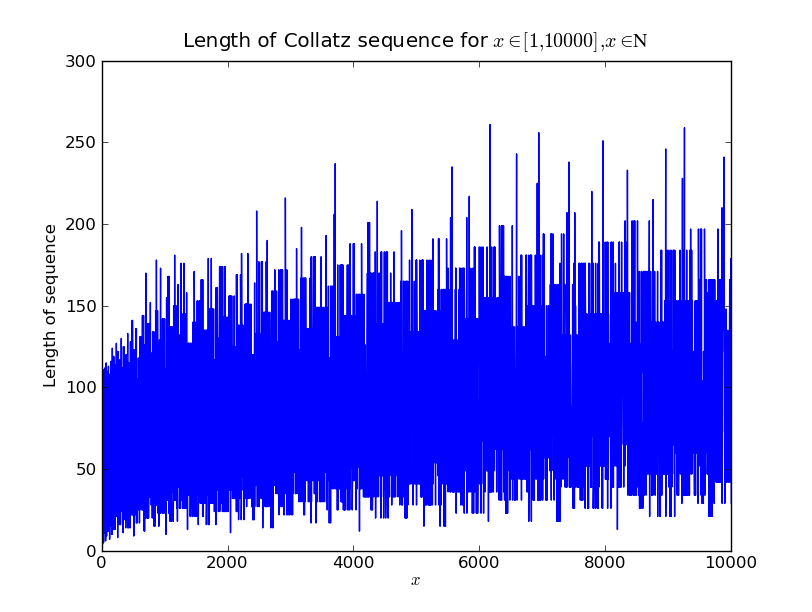
\includegraphics[scale=0.5]{col10000.png}
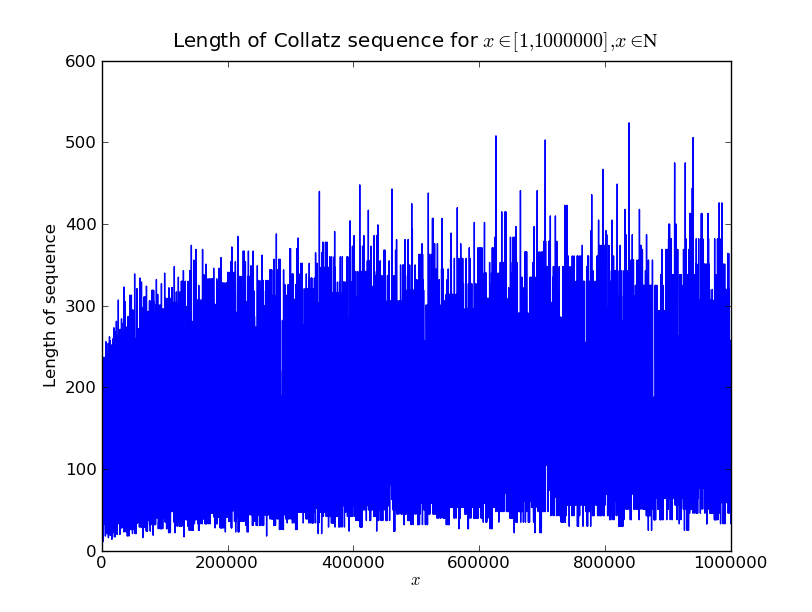
\includegraphics[scale=0.5]{col1000000.png}

There are regularities in these plots. Moving from the interval of [1,100] to
[1,1000000] looks almost like zooming out on a fractal. Each plot is punctuated
by a dozen or so rather large spikes, indicating where particular values have
an especially
long Collatz sequence. Looking at any particular plot, the size of the spikes
generally grows from left to right, but the growth is small. The
spikes look to be fairly evenly far apart.

\section{}
The given statement is false. $g(x)$ is not a primitive recursive function,
because there is no way to bound the time required to compute $n$. As the
Collatz function is applied successively, the input may grow or shrink in no
predictable pattern. If $g(x)$ is implemented recursively, then there
will be no steadily decreasing variable that is given as input into successive
recursive calls, and therefore by definition of $PRIM$, $g(x)$ cannot be in
$PRIM$.

\section{}
An acceptor for $S$ would successively perform the Collatz function. If it
eventually
reached 1, i.e. some $n$ were found such that $f^{(n)}(x)=1$, it would halt and
return YES. Iff an $x$ such that $x \notin S$ were
given to it as input, it would not halt.

\vspace{1em}

We can make no recognizer for $S$ as long as the Collatz problem remains open.
While an acceptor for $S$ is easy to imagine, we can make no rejector
(and therefore no recognizer) for it because we do not know if
$\bar S = \emptyset$. Iff the nature of
$\bar S$ is discovered, and it is computable, and a way to compute it is
discovered, then a recognizer for $S$ can be made. Therefore, whether or not
$S$ has a recognizer is also an open problem pending further insight.

\end{document}
